\documentclass[a4paper,10pt]{report}
\usepackage[utf8]{inputenc}
\usepackage{graphicx} 

% Title Page
\begin{document}

\begin{titlepage}
    \centering
        {\bfseries\Large
        Kaggle Titanic competition\\
        March 2015
        
    }  
     \vfill
     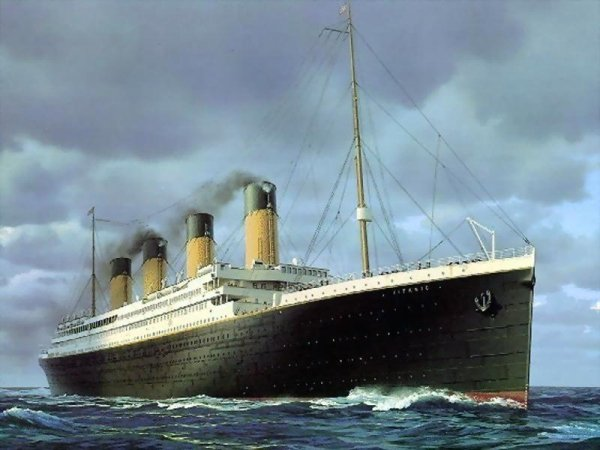
\includegraphics[width=10cm]{titanic.jpg} % also works with logo.pdf
    \vfill
    {\bfseries\Large

        Nicolas Legroux - Hugo Braun\\
        \vskip2cm
        INF582
    }    
    \vfill
   
  
\end{titlepage}

\section*{Introduction}
The Titanic Kaggle competition defines a data science challenge : By using a few features on the passengers onboard
(Name, Age, Family characteristics...) and a train dataset, we have to predict if a passenger has died during the sinking. 
To solve the problem, we tried different approaches, by using various classifiers and performing features engineering,
which lead us to a final score of 0.82297

\section{Input data}
\subsection{Structure}
The input data is separated in two parts : the train data, which contains the 'survived' information, and the test data
on which we have to apply our prediction algorithm.
The data contains the following values :
\begin{enumerate}
 \item PassengerId 
 \item Pclass : the passenger's class in the ship
 \item Name : Contains many informations, like the Surname, the Title (Mr., Mrs., etc...) and the maiden name for a married woman
 \item Sex
 \item Age 
 \item SibSp : Number of siblings aboard
 \item Parch : Number of parents/children aboard
 \item Ticket : String that describes the ticket number
 \item Fare : Price paid for the ticket (a ticket can be shared)
 \item Cabin
 \item Embarked : Port where the passenger embarked
\end{enumerate}

Some features were missing values. The first step was to prepare the data

\subsection{Preparing the data}

\section{Tools}
\subsection{Cross validation}
We implemented a cross validation in order to get some feedback about our models without using Kaggle, using 10% 
of the train data for the test. The results were actually quite surprising : while we always had 
high cross validation score (around 0.88), the result in Kaggle was really above that number.
With our final model we even had a 0.99 cross validation score, corresponding to a 0.81 score on Kaggle. 
This would led us think that the data wasn't randomly splitted between the test and the train data. 

\subsection{Parameters optimisation}
In order to improve our classifiers we tried different methods. One of them was using the sklearn 
capacities of RandomizedSearchCV. This function tries different parameters value in a predefined range 
and returns the most promising ones. Unfortunately, that method didn't really help us to get a better score.

\subsection{Learning curve}
In order to indicate us the bias and variance of our classifiers we used learning curves. This helped us 
noticed the high variance of our decision tree and led us to use a forest.


\section{Classifiers}
\subsection{First decision tree}
We first started with a very simple decision tree. We limited its to 3, and we used only the features directly present
in the data. This decision scored a score of 0.77, which is just above the simple `Gender` approach, but allowed us to 
get into the problem. \\
The tree predicted well the 'easy' profiles : man or woman, class, etc. We now had to find a way to solve the 'hard' cases. 

\subsection{Adding new features (1/2)}
In order to improve our score, we decided to do some feature engineering. At that step, we created the features :




\begin{enumerate}
 \item Title (keeping all of them)
 \item Surname for family above 2 members
 \item Deck
 \item Cabin number
\end{enumerate}

We then decided to use a random forest to use those new features. We were thinking that for instance the Surname feature 
would be useful only with a lot of weak classifiers. We got a score above 0.78 by using that forest. \\
We then tried to improve our use of those features : We merged different categorical values together (like Mme and Mrs, or 
all the superior titles into one). We also created dummies for values like Deck, if a deck in particular had an impact.
All these modifications got us to slightly improve the score. We could noticed in a DecisionTree (depth 3) that for instance the Deck E 
played a special role in the sinking.\\
We then used the 'GroupID' feature. The idea behind that feature is the same idea that behind families : We can expect
that the people who were traveling together were at the same place than the accident occured. By using that feature, we managed
to get above the score of 0.79.

\subsection{Adding new features (2/2)}

\subsection{Bagging}
To that point, we only used trees or forest. We tried other classifiers, like Logistic Regression (with 
only dummy features), GradientBoosting or Extra trees. The idea is that a classifier can be better than 
an other one in a particular situation. To combine the result of all the classifiers used, we finally 
used a DecisionTree.

\begin{figure}[h!]
  \centering
    
      \includegraphics[width=14cm]{finalTree.png}
  \caption{Final decision tree}
\end{figure}

That method got us a score of about 0.8. It did not improve our score, but finest 

\end{document}          
